\documentclass[tikz, border=2pt]{standalone}
\usepackage{amsmath}

\begin{document}
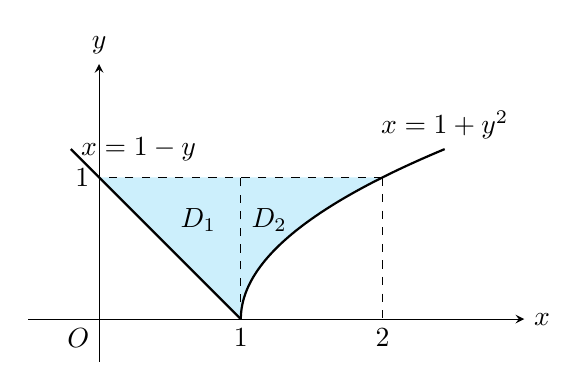
\begin{tikzpicture}[scale=1.8, >=stealth]
    % 填充积分区域 D (由直线 x=1-y、抛物线 x=1+y^2 和水平线 y=1 围成)
    \fill[cyan!20] (1,0) -- plot[domain=0:1, variable=\y, smooth, samples=50] ({1+\y^2},\y) -- (0,1) -- cycle;

    % 画坐标轴
    \draw[->] (-0.5,0) -- (3.0,0) node[right] {$x$};
    \draw[->] (0,-0.3) -- (0,1.8) node[above] {$y$};

    % 画直线 x = 1 - y (稍作延长)
    \draw[thick] (1,0) -- (-0.2,1.2) node[right] {$x=1-y$};
    % 画抛物线 x = 1 + y^2 (稍作延长)
    \draw[thick, domain=0:1.2, variable=\y, smooth, samples=50] plot ({1+\y^2},\y) node[above] {$x=1+y^2$};

    % 画辅助虚线 (从点 (2,1) 向坐标轴)
    \draw[dashed] (2,1) -- (2,0) node[below] {$2$};
    \draw[dashed] (2,1) -- (0,1) node[left] {$1$};
    \draw[dashed] (1,0) -- (1,1) ;
    % 标注 x 轴上的 1
    \draw[dashed] (1,0) -- (1,0.1); % 只是为了让节点对齐，可省略
    \node[below] at (1,0) {$1$};
    % 标注原点
    \node[below left] at (0,0) {$O$};

    % 标注区域 D
    \node at (0.7,0.7) {$D_1$};
    \node at (1.2,0.7) {$D_2$};
\end{tikzpicture}
\end{document}